\documentclass[10pt, AMS Euler]{article}
\textheight=9.25in \textwidth=7in \topmargin=-.75in
\oddsidemargin=-0.25in
\evensidemargin=-0.25in
\usepackage{url}  % The bib file uses this
\usepackage{graphicx} %to import pictures
\usepackage{amssymb, amsmath}
\usepackage{amsthm, concrete, multicol, color, wasysym}
\usepackage{tcolorbox}
\usepackage{tikz}
%\usepackage[normalem]{ulem} %for strikethrough (\sout{blah})
%\usepackage{tikz}
\usepackage{pgfplots}
\usepackage{array}

% adding hyperlinks
\usepackage{hyperref}

% for adding a ^ symbol as text
\usepackage{textcomp} % for \textasciicircum command

% for highlighting
\usepackage{soul}
\usepackage{xcolor}
\usepackage[utf8]{inputenc}
\usepackage{graphicx}

% for inserting code block (kinda)
\usepackage{listings}
\lstdefinestyle{python}{ 
    basicstyle=\ttfamily\footnotesize,
    breaklines=true,
    captionpos=b,
    commentstyle=\color{green},
    keywordstyle=\color{blue},
    numberstyle=\tiny\color{gray},
    stringstyle=\color{orange},
    language=Python,
}

\usetikzlibrary{shapes}
\usetikzlibrary{matrix}
\pgfplotsset{compat=1.14}
\pgfplotsset{rachel style/.append style={axis x line=middle, axis y line=
		middle, xlabel={$x$}, ylabel={$y$}}}
\pgfplotsset{time style/.append style={axis x line=middle, axis y line=
		middle, xlabel={$t$}, ylabel={$f(t)$}}}
\usetikzlibrary{arrows.meta}

% The following is needed for the figures
\usepackage{subfig}
\usetikzlibrary{positioning}
\usepackage{caption}
\usepgfplotslibrary{fillbetween}
%\numberwithin{figure}{section}
\captionsetup{width=.5\textwidth}
\pgfplotsset{
	cartesian style/.append style={axis x line=middle,
		axis y line= middle,
		xlabel={$x$}, ylabel={$y$}},
	midpoint segments/.code={\pgfmathsetmacro\integralsegments{#1}},
	midpoint sum/.style args={#1:#2}{
		ybar interval,
		domain=#1+((#2-#1)/\integralsegments)/2:#2+((#2-#1)/\integralsegments)/2,
		samples=\integralsegments+1,
		x filter/.code=\pgfmathparse{\pgfmathresult-((#2-#1)/\integralsegments)/2}
	}
}
% End of figures stuff

% A website with loads of examples:
% http://pgfplots.sourceforge.net/gallery.html

\usetikzlibrary{calc}


\setlength{\intextsep}{5mm} \setlength{\textfloatsep}{5mm}
\setlength{\floatsep}{5mm}


%%%%  SHORTCUT COMMANDS  %%%%
\newcommand{\ds}{\displaystyle}
\newcommand{\Z}{\mathbb{Z}}
\newcommand{\arc}{\rightarrow}
\newcommand{\R}{\mathbb{R}}
\newcommand{\N}{\mathbb{N}}
\newcommand{\Q}{\mathbb{Q}}
\newcommand{\C}{\mathbb{C}}
\newcommand{\stirling}[2]{\genfrac{\{}{\}}{0pt}{}{#1}{#2}}
\newcommand{\primes}{\mathscr{P}}

%%%%  footnote style %%%%

\renewcommand{\thefootnote}{\fnsymbol{footnote}}

\pgfplotsset{compat=newest}

\begin{document}
	
	
	\noindent{\bf \large Discrete Math 2: Experience One}\\
    \noindent{\bf \large Brighton Ellis; Ann Marie Humble; Nate Stott} \\
	
	\noindent{\bf  Rules:} Complete the following problems by working in groups of at most three, and submit solutions (one document per group) typeset using \LaTeX by blah blah blah.\\
	
	
	
	\noindent {\bf Harmonic Numbers.}  Recall that the {\bf harmonic series} is the series whose terms are the reciprocals of positive integers, and that we defined the {\bf $n^{\mbox{th}}$ harmonic number} $H_n$ to be 
	$$H_n = \sum_{i = 1}^n \frac{1}{i}.$$
	Their name supposedly comes from the fact that a tone with wavelength $1/n$ is the \emph{$n^{\mbox{th}}$ harmonic} of a tone whose wavelength is $1$.  
	
	{\bf Card Trick.}  The numbers $H_n$ arise naturally in simple situations.  
	
	Suppose you have $n$ cards and a table.  Create the largest possible overhang by stacking the cards up over the table's edge (see the figure below for clarification).
	
	\begin{center}
		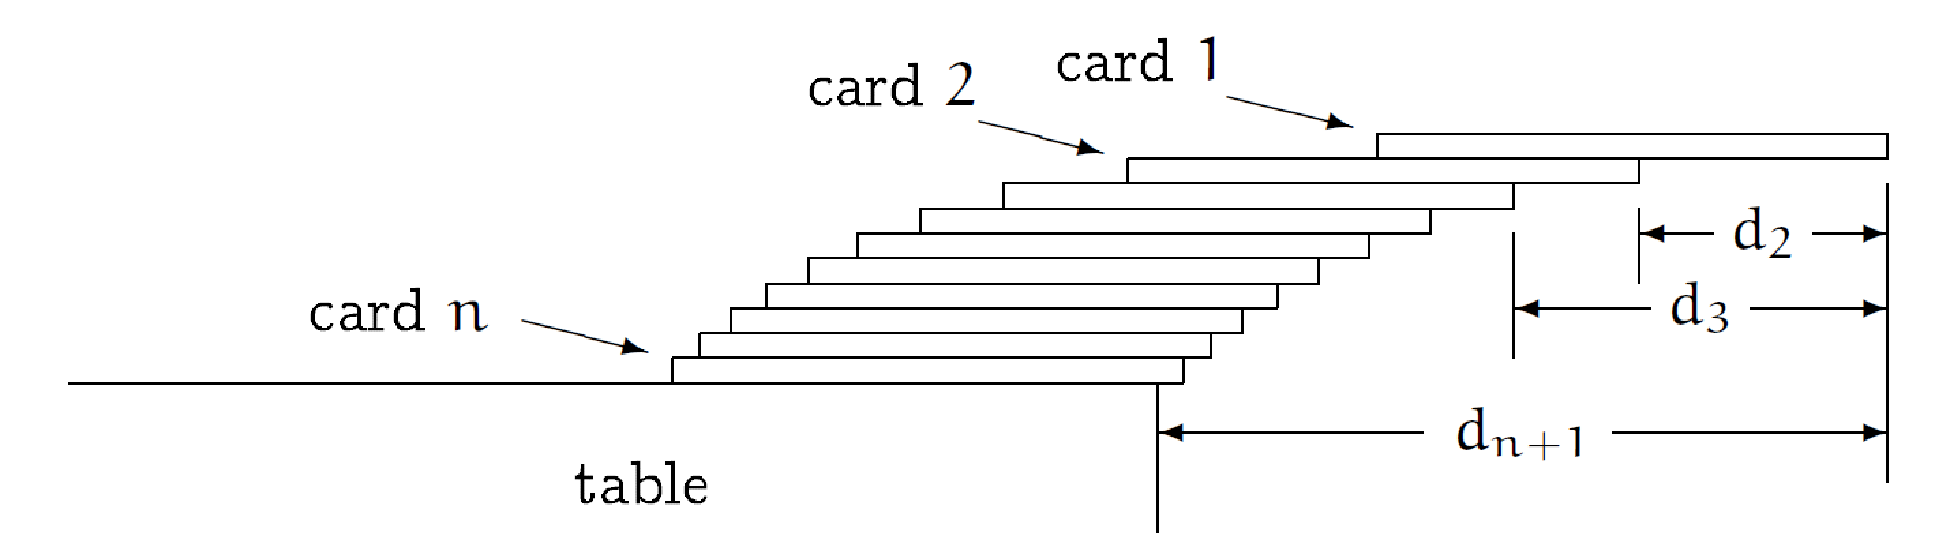
\includegraphics[scale=0.4]{Figures/Overhanging_Cards.pdf}
	\end{center}
	
	Assume the edges of the cards are parallel to the edge of the table (we cannot rotate the cards to make corners stick out further), and assume each card is $2$ units long (this will make calculations a bit easier). \\
	
	\noindent\underline{{\bf Problem 1:}} Determine with proof the maximum overhang you can achieve with $52$ cards, measuring in terms of card lengths.\\
	
	\textsf{Set-up:} Referring to the figure for clarification, put $d_k$ equal to the distance from the extreme edge of the top card to the corresponding edge of the $k^{\mbox{th}}$ card from the top.  So, $d_1 = 0$, and $d_{k+1}$ should be the center of gravity of the first $k$ cards.  
	
	Note that the center of gravity of $k$ objects with respective weights $w_1, \dots, w_k$ and with respective centers of gravity at positions $p_1, \dots, p_k$, is at position 
	$$\frac{w_1p_1 + \cdots + w_kp_k}{w_1 + \cdots + w_k}.$$
	Assume the cards have homogeneous density and equal weight.  
	
	Derive the recurrence 
	\begin{eqnarray*} kd_{k+1} &=& k + d_1+\cdots +d_{k-1}+d_k, \;\;\;\; k \geq 0;\\
		(k-1)d_k &=& k -1 + d_1+ \cdots + d_{k-1}, \;\;\;\; k \geq 1.
	\end{eqnarray*}
	Deduce $$d_{k+1} = d_k + \frac{1}{k}, \;\;\;\mbox{ and hence } \;\;\;d_{k+1} = H_k.$$

    Subtract the second recurrence from the first:\\

    $$kd_{k+1} = k + d_1 + d_2 + ... + d_{k-1} + d_k$$
    $$(k-1)d_k = k-1+d_1+d_2+...+d_{k-1}$$ \\
    Most of the right-hand terms will cancel out, leaving us with:\\

    $$kd_{k+1}-kd_k+d_k=1+d_k$$\\
    $$kd_{k+1}-kd_k=1$$\\
    $$d_{k+1}-d_k=\frac{1}{k}$$\\
    $$d_{k+1}=d_k + \frac{1}{k}$$\\
	
	
	In class we proved (or will prove) that the harmonic series ($H_n$ with $n \to \infty$) 
	\emph{diverges} (meaning that if you specify some, even huge-a\$\$, number $M$, you can find an $n$ so that $H_n> M$).  
	The proof that the harmonic series diverges showed (will show) that (with base of logarithm being $2$)
	$$\frac{\left\lfloor \log{n}\right\rfloor +1}{2} < H_n \leq \left\lfloor \log{n}\right\rfloor +1;$$
	so, the proof method allows to determine $H_n$ within a factor of $2$. 
	But a better bound can be had.  
	
	\begin{center}
		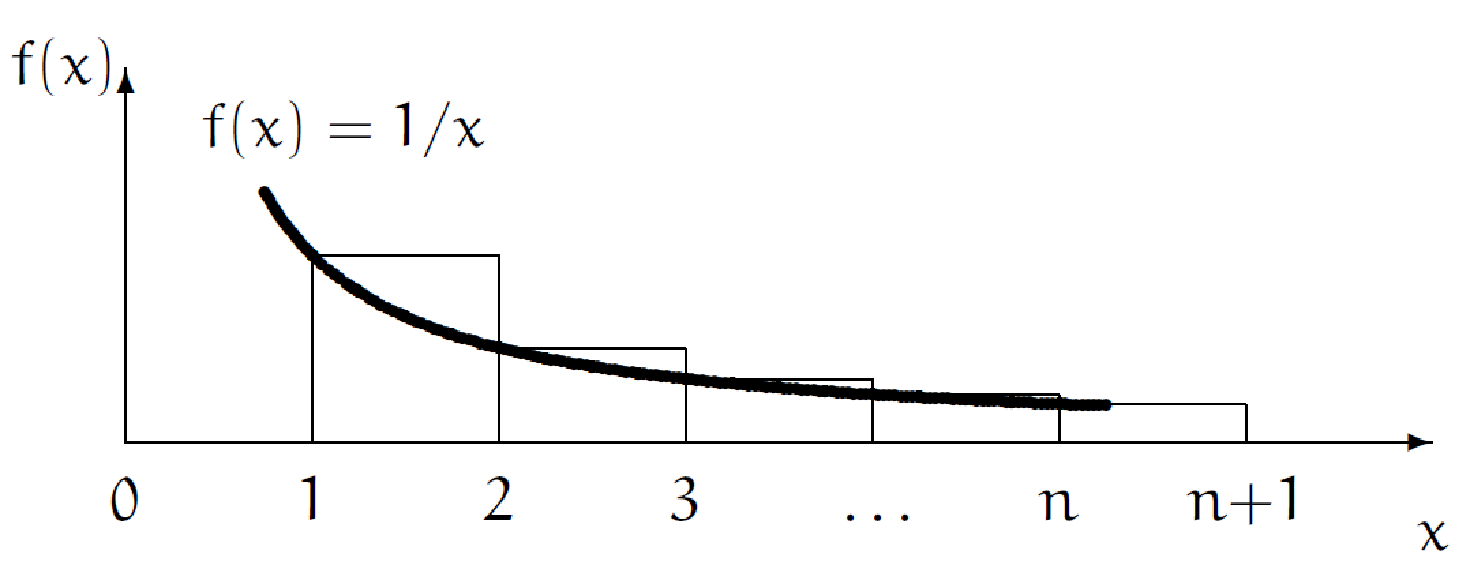
\includegraphics[scale=0.4]{Figures/Harmonic_Left.pdf}
	\end{center}
	
	The natural logarithm is defined as the area under the curve $y = 1/x$; the area between $1$ and $n$ is less than the area of the $n$ rectangles in the figure above. 
	So $$\int_1^n \frac{dx}{x} = \ln{n} < H_n.$$
	But placing the rectangles differently, as in the figure below, gives 
	$$\ln{n} < H_n < \ln{n}+1, \;\;\;\; \mbox{ for $n > 1$.}$$
	\begin{center}
		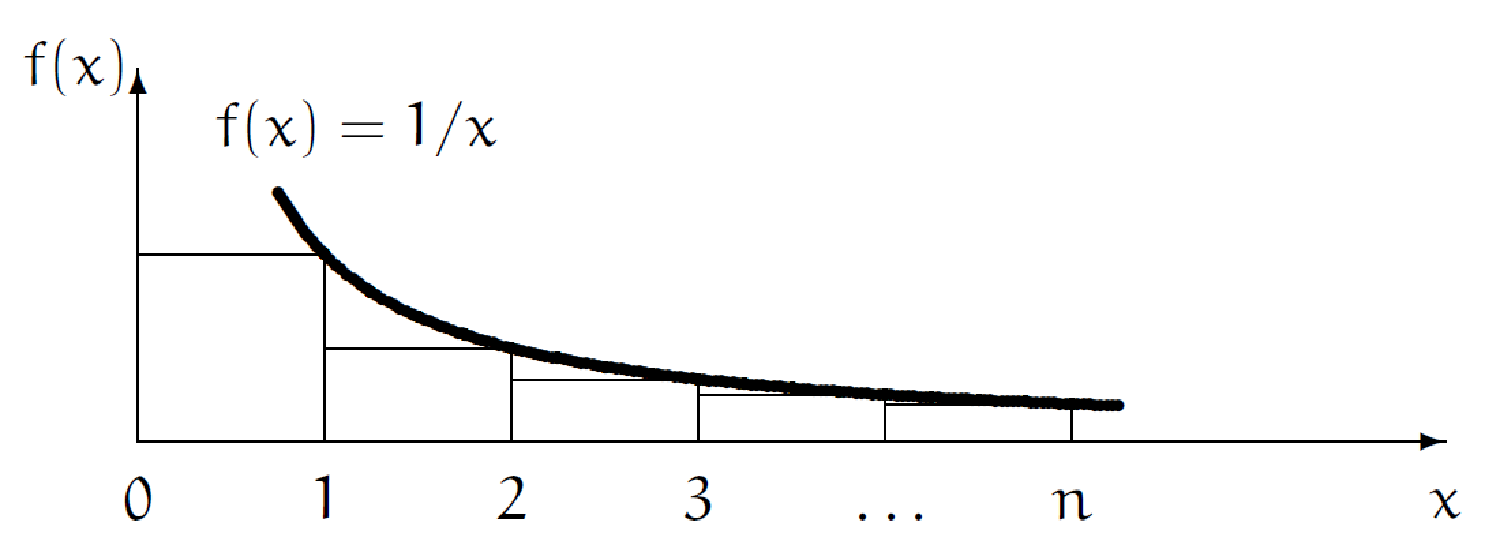
\includegraphics[scale=0.4]{Figures/Harmonic_Right.pdf}
	\end{center}
	Now, we now know $H_n$ within an error of at most $1$. 
	But we can do better.\\

     % TODO: continue problem 1
     % notes from hive mind:
     we can use the plug and chug method by finding the 53$^{rd}$ harmonic number and that should give us the value of the max hang over length of 52 cards. 
     \\
     %Current notes transcribed to here:

        We've already established that a low approximation for $H_n$ is $ln(n)$. In class we talked about how $\gamma$ is a constant for the area of $H_n$ that isn't under the curve $1/x$, and thus is left out when we take $ln(n)$. So all that remains to do is find $ln(n) + \gamma$, which will give us an approximation for $H_n$. The precision of this approximation is only limited by our approximation of $\gamma$.
     
        \begin{align*}
            n = 1000000 \\ 
            H_n = 14.392726722864989 \\ 
            \gamma + ln(n) = 14.392726272863225\\
            n = 51 \\
            H_n = 4.518813181466678 \\
            \gamma + ln(n) = 4.509041347623278\\
            n = 52 \\
            H_n = 4.538043950697447 \\
            \gamma + ln(n) = 4.5284594334803785\\
            n = 53 \\
            H_n = 4.556911875225749 \\
            \gamma + ln(n) = 4.547507628451074\\
            \text{This is our answer}\\
            H_n = \gamma + ln(n) \\
        \end{align*}
% problem 1 has been proofread by Brighton, looks good

        



	
	\noindent\underline{{\bf Problem 2:}} Derive the power series 
	\begin{eqnarray}\ln\left(\frac{x}{x-1}\right) = \frac{1}{x} + \frac{1}{2x^2}+\frac{1}{3x^3} + \frac{1}{4x^4} + \cdots, \label{logseries}\end{eqnarray}
	and deduce from (\ref{logseries}) the following relationship:
	\begin{eqnarray*} \ln{n} - \ln{1} & = & \sum_{k =2}^n \left(\frac{1}{k} + \frac{1}{2k^2} + \frac{1}{3k^3} + \frac{1}{4k^4} + \cdots  \right) \\
		& = & \left(H_n - 1 \right) + \frac{1}{2}\left(H_n^{(2)} - 1 \right) + \frac{1}{3}\left(H_n^{(3)} -1 \right) + \frac{1}{4}\left(H_n^{(4)} -1\right) + \cdots,
	\end{eqnarray*}
	where the notation $H_n^{(r)}$ means $\ds \sum_{k = 1}^n \frac{1}{k^r}$, the {\bf $r^{\mbox{th}}$ order harmonic number}. \\
	
	
	\noindent{\bf Note:} Taking the limit $n \to \infty$ of the $r^{\mbox{th}}$ order harmonic number and we have what is now called the ``\emph{Riemann zeta function}'' 
	$$\zeta(r)  = \lim_{n \to \infty} H_n^{(r)} = \sum_{k \geq 1}\frac{1}{k^r}.$$
	It perhaps ought to be called the ``\emph{Euler zeta function}'' when $r$ is a real number, but that's another story. 
	Riemann studied $\zeta(r)$ and its \emph{analytic continuation} into the complex plane, allowing $r$ to be complex. and discovered many astonishing properties of the function including some that have to do with the distribution of prime numbers.  
	The ``\emph{Riemann hypothesis}'' (should be the ``\emph{Riemann conjecture}'') is that if $\zeta(r) = 0$, then the real part of $r$ is equal to $1/2$. 
	There is a \$1M bounty on the conjecture. \\ 
	
	Anyway, from what was derived from (\ref{logseries}), we have 
	$$H_n - \ln{n} = 1 - \frac{1}{2}\left(H_n^{(2)} - 1 \right) - \frac{1}{3}\left(H_n^{(3)} -1 \right) - \frac{1}{4}\left(H_n^{(4)} -1\right) - \cdots.$$
	As $n \to \infty$, the right-hand side becomes the limiting value 
	$$1 - \frac{1}{2}\left(\zeta(2) - 1 \right) - \frac{1}{3}\left(\zeta(3) -1 \right) - \frac{1}{4}\left(\zeta(4) -1\right) - \cdots,$$
	which is now known as \emph{Euler's constant} and gets denoted by the Greek letter $\gamma$. 
	What you've just worked through is what Euler did, and it establishes the relationship 
	$$\lim_{n \to \infty}\left(H_n - \ln{n}\right) = \gamma.$$

 % TODO: Complete Problem 2

    First, to derive the power series, begin with the FGF, $\frac{1}{1-x}$. The FGF gives us the sequence of all 1's. From there, take $-\ln{1-x}$, which gives us the sequence $x + \frac{x^2}{2} + \frac{x^3}{3} + ...$. Now all we need to do is move every x to the denominator and we'll have something that looks just like the power series above. To do this, replace x with $x^{-1}$, and then simplify:\\

    $-\ln(1-\frac{1}{x})=\frac{1}{x} + \frac{1}{2x^2} + \frac{1}{3x^3} +...$\\

    $-\ln{\frac{x-1}{x}}=\frac{1}{x} + \frac{1}{2x^2} + \frac{1}{3x^3} +...$\\
    
    $\ln{\frac{x}{x-1}}=\frac{1}{x} + \frac{1}{2x^2} + \frac{1}{3x^3} +...$\\

    This is the generating function we've been looking for.\\
    
    Next, notice that $\ln{\frac{x}{x-1}}$ is the same thing as $\ln{x} - \ln{x - 1}$. Consider adding this to itself an egregious number of times (starting at $n=2$):\\

    $\ln{2} - \ln{1} = \frac{1}{k} + \frac{1}{2k^2} + \frac{1}{3k^3} + \frac{1}{4k^4} + \cdots$\\
    $+\ln{3} - \ln{2} = \frac{1}{k} + \frac{1}{2k^2} + \frac{1}{3k^3} + \frac{1}{4k^4} + \cdots$\\
    $+\ln{4} - \ln{3} = \frac{1}{k} + \frac{1}{2k^2} + \frac{1}{3k^3} + \frac{1}{4k^4} + \cdots$\\
    $...$\\
    $+\ln{x} - \ln(x - 1) = \frac{1}{k} + \frac{1}{2k^2} + \frac{1}{3k^3} + \frac{1}{4k^4} + \cdots$\\
    $= \ln(x)-\ln(1) = \sum_{k =2}^n \left(\frac{1}{k} + \frac{1}{2k^2} + \frac{1}{3k^3} + \frac{1}{4k^4} + \cdots  \right)$\\
    
    And thus, the relationship is deduced. Tadah!\\
    % WE GOTTA ADD ANYTHING ABOUT H_n here???
% problem 2 has been proofread by Brighton, looks good, I don't think we need to add anything about H_n
 
	\noindent\underline{{\bf Problem 3:}} Use a computer algebra system (which will have very good approximations for $\zeta(r)$) to compute $\gamma$ to at least $10$ digits of accuracy. \\ 
 
% TODO: Complete Problem 3 
We as a group of nerds... I mean computer Science majors, decided to write our own program for computing gamma. We imported (used somebody else's version) zeta which has been checked for extended approximations to run our calculations. We then provide a value into the gamma function which gives a closer approximation with the higher the input value.  The $f(x)$ function then calculates the value of the Euler-Mascheroni constant (gamma) using the Riemann zeta function and prints the result. 
    - Python Code - \\
    \begin{lstlisting}[style=python]
    from scipy.special import zeta 
    def main(): 
        print(gamma(1000)) 
    def gamma(x): 
        return 1 + f(x) 
    def f(x): 
        sum = 0
        for n in range(2, x): 
            sum -= (1 / n) * (zeta(n) - 1) 
        return sum 
    if __name__ == "__main__": 
        main() 
    \end{lstlisting}
    - Output - \\
    $0.577215664901533$ \\
% problem 3 has been proofread by Brighton, looks good. explanation of python code added, someone check that I explained it properly???



	\noindent{\bf Frustrated Caterpillar.}  You and a friend have a meter-long rubber\footnote{... or some sort of material that has the mystical properties required for this problem} band and decide to mess with a caterpillar named Ting.  
	Ting is at one end of the rubber band and you and your friend are at either end of the rubber band.  Your friend remains stationary, and releases Ting who can crawl at 1 centimeter per minute.  Ting heads toward the other end of the rubber band, where you are (because you have a caterpillar treat) and you stretch the rubber band  1 meter at the end of the each minute.  Ting keeps their relative position on the rubber band as you stretch it (so, at the end of the first minute, after Ting has advanced $1$ cm and is $1\%$ from the start and $99\%$ from you, and you stretch the rubber band to $2$ meters, Ting will be $2$ cm from the starting point and $198$ cm from you). \\
	
	\noindent\underline{{\bf Problem 4:}} Determine with proof how long it will take Ting to reach you.  (Use $\gamma$ from the previous part.)\\ 

At the beginning when the rubber band is only 1 meter long and Ting crawls 1 cm for the first time, Ting is 1 percent of the way across the rubber band. After the rubber band is stretched, Ting is now 2 cm along a 2 meter long rubber band, so Ting is still 1 percent of the way across the rubber band. When Ting crawls another cm and the rubber band is stretched another meter, Ting is 1.5 percent of the way across the rubber band. This is a harmonic series, as shown by the math below:\\

$$nth = \frac{1}{n}$$ \textasciicircum(this is the percentage moved at the nth minute)
$$\sum_{n=1} \frac{1}{n} \geq 100$$
$$\gamma \approx 0.577215664901533$$
$$\gamma \approx H_n - \ln(n)$$
$$H_n \approx \gamma + \ln(n)$$

Since this is a harmonic series, all we need to do is find $H_n$ where $H_n \geq 100$, because when that happens, Ting will be 100 percent of the way across the rubber band. This can be expressed like so:\\

$$H_n \geq 100 - \gamma$$
$$100 \leq \gamma + \ln(n)$$
$$e^{100 - \gamma} \leq e^{\ln(n)}$$
$$e^{100 - \gamma} \leq n$$
$$e^{100 - 0.577215664901533} \leq n$$
$$1.5092688622 \times 10^{43} \leq n$$
Therefore, without further ado, the final answer is that it will take Ting $1.5092688622 \times 10^{43}$ minutes to reach the end of the rubber band. \\
 
	
	\noindent {\bf Generating Functions.} A {\bf partition of $n \in \Z^+$ into $k$ parts} is an equation of the form $n=\lambda_1 + \lambda_2 + \cdots + \lambda_k$, for some $k$, with $\lambda_1 \leq \lambda_2 \leq \cdots \leq \lambda_k$, and $\lambda_i >0$; each $\lambda$ is a {\bf part}.  The number $k$ of parts may not be specified, in which case the terminology is ``\emph{a partition of $n$}''. 
	
	Define $p(n)$ to be the number of partitions of $n$.  
	For convenience, we take $p(0)$ to be $1$. 
	It might behoove you to verify the sequence $\left(p(n)\right)_{n \geq 0}$ begins 
	$$\left( p(n)\right)_{n \geq 0} = (1,1,2,3,5,7,11,15,22, \dots);$$
	that is, $p(2) = 2, p(5) = 7, p(6)=11,$ and so on. 
	
	Define $\mathcal{E}(x)$ to be the generating function for the sequence $\left(p(n)\right)_{n \geq 0}$; that is 
	$\ds \mathcal{E}(x) = \sum_{n \geq 0}p(n)x^n$. 
	In class it was observed that $$\mathcal{E}(x) = \prod_{k > 0} \frac{1}{1-x^k}.$$
 % problem 4 has been proofread by Brighton, looks good
	
	\noindent \underline{{\bf Problem 5:}}  Define $p_{\mbox{\scriptsize no } 1}(n)$ to be the number of partitions of $n$ with no part equal to $1$.  Prove that $p_{\mbox{\scriptsize no }1}(n) = p(n) - p(n-1).$\\
 
 % TODO: Complete Problem 5
To start off, lets get an idea of what the sequence looks like for $P_{no 1}$\\

    \begin{align*}
        p_{\mbox{\scriptsize no }1}(0) = 1 ,\text{ } & p(0) = 1  \\
        p_{\mbox{\scriptsize no }1}(1) = 0 ,\text{ } & p(1) = 1  \\
        p_{\mbox{\scriptsize no }1}(2) = 1 ,\text{ } & p(2) = 2  \\
        p_{\mbox{\scriptsize no }1}(3) = 1 ,\text{ } & p(3) = 3  \\
        p_{\mbox{\scriptsize no }1}(4) = 2 ,\text{ } & p(4) = 5  \\
        p_{\mbox{\scriptsize no }1}(5) = 2 ,\text{ } & p(5) = 7  \\
        p_{\mbox{\scriptsize no }1}(6) = 4 ,\text{ } & p(6) = 11 \\
        p_{\mbox{\scriptsize no }1}(7) = 4 ,\text{ } & p(7) = 15 \\
    \end{align*}
    The values of the unique partitions above (the right side equation) can be referenced in the "Partition function" section of the following wikipedia page: \href{https://en.m.wikipedia.org/wiki/Integer_partition}{wikipedia page}. \\
    
We can set a base case for $0$ and $1$, and then work with the remaining sequence. We can create a combinatorial argument for this. Assuming that $p_{\mbox{\scriptsize no }1}(n) = p(n) - p(n-1)$, then we can move terms around and get that the combinations with no 1 plus the combinations that do contain ones is equal to the total possible combinations of partitions. We can show this looking at the figure below with $n=5$ as our example:
\begin{align*}
    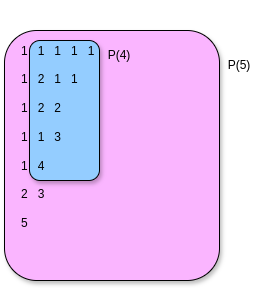
\includegraphics[width=.25\textwidth]{Figures/prob5.png}
\end{align*}

For this case, $7-5=2$ which follows with the sequence we got above, and further shows that the provided relationship is in fact correct. \\
% problem 5 has been proofread by Brighton, looks good
	
	\noindent \underline{{\bf Problem 6:}} Define $p_k(n)$ to be the number of partitions of $n$ with at most $k$ parts.  
	Prove that the generating function for $\left(p_k(n)\right)_{n \geq 0}$ is 
	$$\sum_{n \geq 0} p_k(n)x^n = \frac{1}{(1-x)(1-x^2)(1-x^3)(1-x^4) \cdots (1-x^k)},$$
	and [calculate] $p(27)$ and $p_5(27)$ using the generating function relationships just proved. 
	\\
 % TODO: Complete Problem 6

    For the generating function above, the nth coefficient is the number of ways to partition a set of size n where the largest part of the partition is size k. This is because the generating function is multiplying all the ways to partition a set of size n with no parts larger than 1, all the ways to partition with no parts larger than 2, etc. etc. up to every way to partition with no parts larger than k.\\

    This counts the same thing as the number of partitions of $n$ with at most $k$ parts. If you drew out some partition of dots where each row was a part and the most dots in any row is $k$, this is the number of ways to partition a set of size n with no parts being larger than $k$.\\

    However, if you let the columns represent the partitions instead of the rows, you would have $k$ columns, all of various sizes (since the most dots in any row is $k$). \emph{This} is counting the number of partitions of $n$ with at most $k$ parts, which is what this generating function is supposed to be counting. Therefore, the generating function for $\left(p_k(n)\right)_{n \geq 0}$ is 
	$$\sum_{n \geq 0} p_k(n)x^n = \frac{1}{(1-x)(1-x^2)(1-x^3)(1-x^4) \cdots (1-x^k)}$$.\\


    To find $p_5(27)$, find the 27th coefficient on the generating function, where $(1-x^i)$ has $1 \leq i \leq 5$. This can be done using the following Maxima code:\\

    \begin{verbatim}
        g(x) := product(1-x^i, i, 1, 5);
        f(x) := 1 / g(x);

        taylor(f(x), x, 0, 27);
    \end{verbatim}

    This returns a series, the 27th term of which has the coefficient 480. Therefore, $p_5(27) = 480$.\\

    $p(27)$ is asking us to find the number of partitions of n where n is 27, with at most n parts (because you can't have more than n parts with only n items you're partitioning). Therefore, to find p(27), do the same thing as above but for $1 \leq i \leq 27$. Doing this, the coefficient on the 27th term of the series is 3010. And so, $p(27) = 3010$.\\

% I BELIEVE THIS ^^^ IS CORRECT, IF SOMEBODY WANTS TO CHECK MY WORK THAT'D BE GREAT :)
% confirmed by Brighton and Wikipedia, this is correct. 
 
	\noindent{\bf Catalan Numbers.}  Define $C_n$ to be the number of valid strings of $n$ pairs of parentheses; that is, the empty string is a valid string, and if $A$ and $B$ are valid strings of parentheses, then so are $A(B)$ and $(A)B$. The sequence $\left(C_n\right)_{n \geq 0}$ begins 
	$$\left(C_n\right)_{n \geq 0} = (1,1,2,5,14, \dots ).$$

	\noindent\underline{\bf Problem 7:}  Prove that the numbers $C_n$ can be created via the recurrence relation 
	\begin{align*} C_{n+1} & = C_nC_0 + C_{n-1}C_1 + C_{n-2}C_2 + \cdots + C_1C_{n-1} + C_0C_n \mbox{ for } n \geq 0\\
		C_0 & = 1 
	\end{align*}

 Alrighty then, let's go ahead and get crack-a-lackin! First let's set up the recurrence relation as a sum for visual appeal. 

    $$ C_{n+1} = C_nC_0 + C_{n-1}C_1 + C_{n-2}C_2 + \cdots + C_1C_{n-1} + C_0C_n $$
    $$ C_{n+1} = \sum_{i=0}^n C_{n-i} C_i $$

    $$ C_n = \sum_{i=0}^{n-1} C_{n-i-1} C_i $$
below we will plug in numbers to test our base cases. this is more to prove to ourselves that the recurrence for plain ol' $C_n$ we deduced above does in fact work. 
    $$ C_0 = 1 $$
    $$ C_1 = \sum_{i=0}^{1-1} C_{1-0-1} C_0 = \sum_{i=0}^{0} C_{0} C_0 = C_0 C_0 = 1 $$
    $$ C_2 = \sum_{i=0}^{2-1} C_{2-i-1} C_i = \sum_{i=0}^{1} C_{1-i} C_i = C_1 C_0 + C_0 C_1 = 2 $$
    $$ C_3 = \sum_{i=0}^{3-1} C_{3-i-1} C_i $$
    $$ C_3 = C_2(C_0) + C_1(C_1) + C_0(C_2) $$
    $$ C_3 = 2(1) + 1(1) + 1(2) = 5 $$
    $$ C_4 = \sum_{i=0}^{3} C_{3-i} C_i $$
    $$ C_4 = C_3(C_0) + C_2(C_1) + C_1(C_2) + C_0(C_3) $$
    $$ C_4 = 5(1) + 2(1) + 1(2) + 1(5) = 14 $$

    $$ 1, 1, 2, 5, 14 $$
    It works! So we shall use $ C_n = \sum_{i=0}^{n-1} C_{n-i-1} C_i $ in Problem 8 \\
    \\
	
	\noindent\underline{\bf Problem 8:} Define $C(x)$ to be the generating function for the Catalan numbers; that is, $\ds C(x) = \sum_{n \geq 0}C_nx^n$. Show that $C(x) = \ds \frac{1 - \sqrt{1-4x}}{2x}$. \\

    Define $[n=0]$ to give $1$ if true and $0$ if false

    $$ C_n = \sum_{i=0}^{n-1}C_{n-i-1}C_i + [n = 0] $$

    Define $C(x) = \sum_{n\geq0} C_n x^n$ \\

    $$ C(x) = \sum_{n\geq0} \left( \sum_{i=0}^{n-1} C_{n-i-1}C_i \right)x^n + \sum_{n\geq0} [n = 0] x^n $$

    $$ C(x) = \sum_{n\geq0} \left(\sum_{i=0}^{n-1} C_{n-i-1}C_i \right)x^n + 1 $$

    $$ C_n = \sum_{i=0}^{n-1} C_{n-i-1} C_i = C_{n-1} C_0 + C_{n-2} C_{1} + C_{n-3} C_{2} + ... + C_{2} C_{n-3} + C_{1} C_{n-2} + C_{0} C_{n-1} $$

    $$ C_n^2 = \left(\sum_{i=0}^{n-1} C_{n-i-1} C_i\right) \left(\sum_{i=0}^{n-1} C_{n-i-1} C_i\right)  $$
    $$ = (C_{n-1} C_0 + C_{n-2} C_{1} + ... + C_{1} C_{n-2} + C_{0} C_{n-1}) (C_{n-1} C_0 + C_{n-2} C_{1} + ... + C_{1} C_{n-2} + C_{0} C_{n-1}) $$
    $$ = \sum_{i=0}^{n} C_i C_{n-i} = C_n C_0 + C_{n-1} C_1 + C_{n-2} C_2 + ... + C_2 C_{n-2} + C_1 C_{n-1} + C_0 C_n $$
    
    Well hey, $C_n^2 = C_{n+1}$. That means that $C(x)^2 = \sum_{n\geq0} C_{n+1} x^n$.
    
    $$ C(x)^2 = \sum_{n\geq0} C_{n+1} x^n $$
    $$ x C(x)^2 = \sum_{n\geq0} C_{n+1} x^{n+1} $$
    We have to add $1$ to account for $C_0$
    $$ x C(x)^2 + 1 = C(x) $$
    $$ x C(x)^2 - C(x) + 1 = 0 $$
    Using the quadratic equation to solve for $C(x)$ with $a=x$, $b=-1$, and $c=1$
    $$ C(x) = \frac{1 \pm \sqrt{(-1)^2 - 4x}}{2x} $$
    $$ C(x) = \frac{1 \pm \sqrt{1 - 4x}}{2x} $$
    Because $ C(x) = \frac{1 + \sqrt{1 - 4x}}{2x} $ goes to infinity when approaching 0 we can throw that solution out. The other solution goes to 1 which would satisfy $C_0 = 1$.
    $$ C(x) = \frac{1 - \sqrt{1 - 4x}}{2x} $$
% problem 8 checked by Brighton. can someone else give some explanations between some of the steps above? it's difficult for me to follow
	
	\noindent\underline{\bf Problem 9:} Show that $\ds C_n = \frac{1\cdot 3 \cdot 5 \cdots (2n-1)}{(n+1)!}\cdot 2^n,$
	and hence, finally, that $C_n = \ds \frac{1}{n+1} \binom{2n}{n}$. (This is the most common expression for the $n^{\mbox{th}}$ Catalan number.)\\
     
    $$ C(x) = \frac{1 - \sqrt{1 - 4x}}{2x} $$
    Using Newtons Binomial Theorem! 
    $$ (1+x)^a = \sum_{n \geq 0 } \binom{a}{n} x^n $$
    $$ \sqrt{1 - 4x} = (1+(-4x))^{\frac{1}{2}} = \sum_{n \geq 0 } \binom{\frac{1}{2}}{n} (-4x)^n $$
    So
    $$ C(x) = \frac{1 - \sqrt{1 - 4x}}{2x} = \frac{1 - \sum_{n \geq 0 } \binom{\frac{1}{2}}{n} (-4x)^n }{2x} $$

    When $n=0$, $\binom{\frac{1}{2}}{0} (-4x)^0 = 1 * 1 = 1 $. This means that we can start the summation at $1$ and get rid of the $1$ at the start.
    
    $$ C(x) = -\frac{1}{2}(\sum_{n \geq 1 } \binom{\frac{1}{2}}{n} (-4)^n x^{n-1}) $$
    $$ C(x) = -\frac{1}{2}(\sum_{n \geq 1 } \binom{\frac{1}{2}}{n} (-4)^n x^{n-1}) $$
    Index shift
    $$ C(x) = -\frac{1}{2}(\sum_{n \geq 0 } \binom{\frac{1}{2}}{n+1} (-4)^{n+1} x^n) $$
    
    $$ C_n = -\frac{1}{2} (-4)^{n+1} \binom{\frac{1}{2}}{n+1} $$

    Expanding the binomial coefficient
    $$ \binom{n}{k} = \frac{n^{\underline{k}}}{k!} $$

    $$ C_n = -\frac{1}{2} (-4)^{n+1} \frac{(\frac{1}{2})^{\underline{n+1}}}{(n+1)!} $$
    $$ C_n = \frac{(-1)(-4)^{n+1} (\frac{1}{2})^{\underline{n+1}}}{2(n+1)!} $$

    $$ C_n = \frac{(-1)(-4)^{n+1} ((\frac{1}{2})(\frac{1}{2} -1)(\frac{1}{2} -2)(\frac{1}{2} -3)...(\frac{1}{2} - n + 1)(\frac{1}{2} - n))}{2(n+1)!} $$

    $$ C_n = \frac{(-1)(-4)^{n+1} ((\frac{1}{2})(\frac{1}{2} -1)(\frac{1}{2} -2)(\frac{1}{2} -3)...(\frac{3}{2} - n)(\frac{1-2n}{2}))}{2(n+1)!} $$

    $$ C_n = \frac{(-1)(-4)^{n+1} ((\frac{1}{2})(\frac{-1}{2})(\frac{-3}{2})(\frac{-5}{2})...(\frac{3-2n}{2})(\frac{1-2n}{2}))}{2(n+1)!} $$

    $$ C_n = \frac{(-1)(-4)^{n+1} ((\frac{1}{2^{n+1}})(-1)(-3)(-5)...(3-2n)(1-2n))}{2(n+1)!} $$

    $$ C_n = \frac{(-1)(-4)^{n+1} ((1)
    (-1)(-3)(-5)...(3-2n)(1-2n))}{(2^{n+2})(n+1)!} $$

    $$ C_n = \frac{(-1)(-4)^{n+1} ((-1)(-3)(-5)...(3-2n)(1-2n))}{(2^{n+2})(n+1)!} $$

    $$ C_n = \frac{(-1)^{n+1} (4)^{n+1} (-1)^{n+1} ((1)(3)(5)...(2n-3)(2n-1))}{(2^{n+2})(n+1)(n)!} $$

    $$ C_n = \frac{(2)^{n+1} (2)^{n+1} }{(2^{n+2})(n+1)} * \frac{(1)(3)(5)...(2n-3)(2n-1)}{(n)!} $$

    $$ C_n = \frac{ (2)^{n+1} }{(2)(n+1)} * \frac{(1)(3)(5)...(2n-3)(2n-1)}{(n)!} $$

    $$ C_n = \frac{((1)(3)(5)...(2n-3)(2n-1))}{(n+1)!} \cdot 2^n $$
    There is the first form that is asked for in the question prompt \\
    Now time for the next form
    $$ C_n = \frac{(1)(3)(5)...(2n-1)}{(n+1)!} \cdot 2^n $$

    $$ C_n = \frac{1}{n+1} * \frac{((1)(3)(5)...(2n-1))2^n}{n!} $$

    Working backwards
    
    $$ C_n = \frac{1}{n+1} \binom{2n}{n} $$

    $$ \binom{n}{k} = \frac{n!}{k!(n-k)!} $$

    $$ C_n = \frac{1}{n+1} \frac{(2n)!}{n!((2n)-n)!} $$

    $$ C_n = \frac{1}{n+1} \frac{(2n)(2n-1)(2n-2)(2n-3)(2n-4)...(4)(3)(2)(1)}{(n!)^2} $$
    
    $$ C_n = \frac{1}{n+1} \frac{((2n)(2n-2)(2n-4)...(4)(2))((2n-1)(2n-3)...(3)(1))}{(n!)^2} $$

    $$ C_n = \frac{1}{n+1} \frac{2^n((n)(n-1)(n-2)...(2)(1))((2n-1)(2n-3)...(3)(1))}{(n!)^2} $$  

    $$ C_n = \frac{1}{n+1} \frac{2^n(n!)((2n-1)(2n-3)...(3)(1))}{(n!)^2} $$ 

    $$ C_n = \frac{1}{n+1} \frac{2^n((2n-1)(2n-3)...(3)(1))}{n!} $$

    Well boom there you go they are worked out to be the same thing

    $$ C_n = \frac{1}{n+1} \binom{2n}{n} $$ \\
% Proofread of prob 9 done by Brighton. it's a lot to look at but it is correct. so we good!
	
	\noindent\underline{\bf Problem 10:}  In how many ways can a $2 \times 2 \times n$ pillar be built out of $2 \times 1 \times 1$ bricks?\\
 
    Here is the recurrence relation.
    $$ S_0 = 1 $$
    $$ S_1 = 2 $$
    $$ S_2 = 9 $$
    $$ S_n = 2 S_{n-1} + S_{n-2} + 4 \sum_{i = 2}^n S_{n-i} $$

    We got this recurrence by looking at the layers of blocks and all the combinations of blocks when you consider a number of layers starting from the top.\\ 
    
    If the top layer is all horizontal blocks, then we can shave it off the pillar and look at layer $(n-1)$. And since there are two ways for the top layer of blocks to be made up of only horizontal blocks (both blocks facing North/South, or both blocks facing East/West), we have $2 S_{n-1}$ in the recurrence. If the top layer is all vertical blocks, then we can shave it off the pillar (removing a height of 2 from the pillar) and look at the next flat layer, which is layer $(n-2)$. There is only one way for the top layer to be all vertical blocks, and so we have $S_{n-2}$ in the recurrence. And finally, if the top layer is made of a combination of vertical and horizontal blocks, we don't know how many blocks we'll have to remove before hitting the next flat layer in the pillar. The closest it could be is just below the topmost vertical blocks (hence starting the summation at $i=2$). It could also be that there are no all-horizontal or all-vertical layers in the pillar. This is where the $\sum_{i = 2}^n S_{n-i}$ in the recurrence comes from, because we may end up having to check every layer. And since there are four ways to have a mixed vertical/horizontal top layer (vertical blocks are on the North side, East side, South side, or West side), we multiply this part of the recurrence by 4 to get $4 \sum_{i = 2}^n S_{n-i}$\\.
    
    Make it work for any $n$. Define $S_n=0$ if $n<0$. Define $[n=0]$ to give $1$ if true and $0$ otherwise. \\
    $$ S_n = 2 S_{n-1} + S_{n-2} + 4 \sum_{i = 2}^n S_{n-i} + [n=0] $$
    $$ S_0 = 2 S_{-1} + S_{-2} + 4 \sum_{i = 2}^0 S_{0-i} + 1 = 2(0) + 0 +4(0) + 1 = 1 $$
    $$ S_1 = 2 S_{0} + S_{-1} + 4 \sum_{i = 2}^1 S_{1-i} + 0 = 2(1) + 0 + 4(0) = 2 $$
    $$ S_2 = 2 S_{1} + S_{0} + 4 \sum_{i = 2}^2 S_{2-i} + 0 = 2(2) + 1 + 4(1) = 4 + 5 = 9 $$
    It works! \\
    Define $S(x) = \sum_{n \geq 0} S_n x^n $. \\
    Multiply everything by the summation and $x^n$
    $$ S(x) = 2 \sum_{n \geq 0} S_{n-1} x^n + \sum_{n \geq 0} S_{n-2} x^n + 4 \sum_{n \geq 0} (\sum_{i = 2}^n S_{n-i}) x^n + \sum_{n \geq 0} [n=0] x^n $$
    $$ S(x) = 2 x S(x) + x^2 S(x) + 4 \sum_{n \geq 0} (\sum_{i = 2}^n S_{n-i}) x^n + 1 $$
    $$ S(x) = 2 x S(x) + x^2 S(x) + 4 \sum_{n \geq 0} ( (\sum_{i = 0}^n S_i) - S_n - S_{n-1}  ) x^n + 1 $$
    $$ S(x) = 2 x S(x) + x^2 S(x) + 4 (\sum_{n \geq 0} (\sum_{i = 0}^n S_i) x^n - \sum_{n \geq 0} S_n x^n - \sum_{n \geq 0} S_{n-1} x^n) + 1 $$
    $$ S(x) = 2 x S(x) + x^2 S(x) + 4 ( \frac{1}{1-x} S(x) - S(x) - x S(x) ) + 1 $$
    $$ S(x) = 2 x S(x) + x^2 S(x) + 4 \frac{1}{1-x} S(x) - 4 S(x) - 4 x S(x) + 1 $$
    $$ S(x) - 2 x S(x) - x^2 S(x) - 4 \frac{1}{1-x} S(x) + 4 S(x) + 4 x S(x) = 1 $$
    $$ S(x) ( 1 - 2 x - x^2 - 4 \frac{1}{1-x} + 4 + 4 x ) = 1 $$
    $$ S(x) ( 5 + 2 x - x^2 - 4 \frac{1}{1-x} ) = 1 $$
    $$ S(x) = \frac{1}{ 5 + 2 x - x^2 - 4 \frac{1}{1-x} } $$
    $$ S(x) = \frac{1-x}{(x+1)(x^2-4x+1)} $$
    $$ S(x) = \frac{1-x}{-(x+1)(-x+\sqrt{3}+2)(x+\sqrt{3}-2)} $$
    $$ S(x) = \frac{x-1}{(x+1)(-x+\sqrt{3}+2)(x+\sqrt{3}-2)} $$
    $$ S(x) = \frac{A}{x+1} + \frac{B}{-x+\sqrt{3}+2} + \frac{C}{x+\sqrt{3}-2} $$ 
    \\
    $$ x-1 = A(-x+\sqrt{3}+2)(x+\sqrt{3}-2) + B(x+1)(x+\sqrt{3}-2) + C(x+1)(-x+\sqrt{3}+2) $$
    Cutting to the point after using smart online math tools, $A=\frac{1}{3}$, $B=-\frac{1}{6}$, $C=-\frac{1}{6}$
    $$ S(x) = \frac{\frac{1}{3}}{x+1} - \frac{\frac{1}{6}}{-x+\sqrt{3}+2} - \frac{\frac{1}{6}}{x+\sqrt{3}-2} $$ 
    $$ S(x) = \frac{1}{3} * \frac{1}{x+1} - \frac{1}{6} * \frac{1}{-x+\sqrt{3}+2} - \frac{1}{6} * \frac{1}{x+\sqrt{3}-2} $$ 

    Using the reverse polynomial thing you get

    $$ S(x) = \sum_{n \geq 0} \frac{1}{6} (2(-1)^n + (2-\sqrt{3})^{n+1} + (2+\sqrt{3})^{n+1} ) x^n $$
    $$ S_n = \frac{1}{6} (2(-1)^n + (2-\sqrt{3})^{n+1} + (2+\sqrt{3})^{n+1} ) $$
    Checked for $n=0,1,2,3$\\
    % problem 10 checked by Brighton 
 
	\noindent\underline{\bf Problem 11:}  A form of DNA found stuck to a space probe has been analyzed and found to consist of five different molecules, call them $a,b,c,d,e$.  Research shows that the pairs $cd, ce, ed,$ and $ee$ cannot occur consecutively in a string of this mysterious DNA, but any string without these \emph{forbidden pairs} can occur.  
	So, for example $bbcda$ is not possible, but $bbdca$ is.  How many different mysterious DNA strings of length $n$ are possible?  Note that when $n=2$, there are $21$ different strings because the left and right ends of the string are distinguishable.\\
    
    I shall call the function $P$ for probe. $P$ is the number of different mysterious DNA strings of length $n$ that are possible. 

    These numbers come from a python program. 
    $$ P_0 = 1 $$ 
    $$ P_1 = 5 $$
    $$ P_2 = 21 $$
    $$ P_3 = 89 $$
    $$ P_4 = 377 $$
    $$ P_5 = 1597 $$
    $$ P_n = 4P_{n-1} + P_{n-2} $$

    % The recurrence above comes from the following reasoning:\\

    Here is our reasoning for the ratio above:

    Condition on the last letter in the sequence. The following is a table of possible letters:\\

    \begin{table}[h]
    \centering
    \begin{tabular}{|c|c|c|}
        \hline
        \textbf{Second-to-last Letter} & \textbf{Last Letter} \\
        % \hline
        a, b, c, d, e & a \\
        \hline
        a, b, c, d, e & b \\
        \hline
        a, b, c, d, e & c \\
        \hline
        a, b, d & d \\
        \hline
        a, b, d & e \\
        \hline
    \end{tabular}
    \end{table}

    a, b, and c have no constraints on the letters that can come before them, so a, b, and c each have 5 possible preceding letters.\\

    d and e can only have a, b, and d come before them. a and b are unrestricted with five possible letters before them each, so d and e collectively have $5 * 4 = 20$ possible letters for the $(n-1)$th letter. But we had to go one layer deeper to get that number, so divide 20 by 4 (two for d as last letter and two for e as last letter), which gives us another 5 for the $(n-1)$th letter.\\

    d is restricted, so if the last letter is d or e and the second-to-last letter is d, then the third-to-last letter can be a, b, or d. Again, a and b are unrestricted with 5 possible preceding letters. So $5 * 4 = 20$. But divide that by 4 (two for d two for e) and you get 5. This counts toward $(n-2)$ because now we're looking at third-to-last letters.\\

    Thus, the ratio of $4P_{n-1}+P_{n-2}$.\\

    % Now think about possibilities for the third-to-last letter. Second-to-last and last letter combinations aa, ba, ca, ab, bb, cb, ac, bc, cc collectively have 45 possible sequences for the third-to-last letter (five possible sequences for each second-to-last and last letter pair). These are $P_{n-1}$ because we only have to look at the last and second-to-last letters to know that there are no restrictions on third-to-last letters for these sequences.\\

    % Second-to-last and last letter combinations da, ea, db, eb, dc, ec have potential problems, because only a, b, and d are allowed to precede d and e. Thus, we have restrictions on what the third-to-last letter can be. If the third-to-last letter is a or b, we have no restrictions on what the fourth-to-last letter is. Here are those sequences (in order of third-to-last, second-to-last, and last) ada, bda, aea, bea, adb, bdb, aeb, beb, adc, bdc, aec, bec. Each one of these sequences has 5 possibilities for what letter can precede them, making 60 possibilities total. However, since we only had 6 sequences (of second-to-last and last) to begin with, divide these possibilities by 6. That makes 10 additional possibilities for $P_{n-1}$.\\

    % What we did not account for in the last paragraph is that d or e can also be preceded by d without making an invalid sequence. Let's count up the possible third-to-last letters when this is the case. We have the sequences (in order of third-to-last, second-to-last, and last letter) dda, dea, ddb, deb, ddc, dec. Now we have to go one layer deeper to see what letters can precede these sequences. We know that d can be preceded by a or b without restriction on what comes before that, meaning that the fourth-to-last letters for these sequences, without restriction on what comes before, are adda, bdda, adea, bdea, addb, bddb, adeb, bdeb, addc, bddc, adec, bdec. Each of these sequences has five possible letters that can precede them, making 60 possibilities total. And just like last time, since these come from 6 sequences originally, we have to divide this number by 6, making 10 additional possibilities for the fourth-to-last letter. However, since we have already defined $P_{n-1}$ as pertaining to the possibilities for the second-to-last letter, this number has to apply to $P_{n-2}$ instead of $P_{n-1}$.\\

    % Now we need to look at the possible third-to-last letters when the last letter in the sequence is d or e and the second-to-last letter in the sequence is a or b. Since a and b have no restriction on what can come before them, the sequences (in order of second-to-last and last) ad, bd, ae, be have 20 possibilities for the third-to-last letter. Dividing this by four, because these came from four sequences, we get 5 additional possibilities for $P_{n-1}$.\\

    % And finally, if we look at the possible third-to-last letters when the last letter in the sequence is d or e, and the second-to-last letter in the sequence is d, we get the sequences add, bdd, ade, bde. That gives us 20 possibilities for the third-to-last letter, but since the last letter was d or e, we divide this by the number of sequences we started with, giving us 5. And since we had to go one level deeper to find a valid sequence without restriction, those 5 possibilities apply to $P_{n-2}$.\\

    % Now if we add together every $P_{n-1}$ and $P_{n-2}$, we get:\\

    % $45 P_{n-1} + 10 P_{n-1} + 5 P_{n-1} = 60 P_{n-1}$\\
    % $10 P_{n-2} + 5 P_{n-2} = 15 P_{n-2}$\\

    % And if we simplify this ratio, we get $4P_{n-1} + P_{n-2}$, and thus the ratio in our sequence.\\
    

    Make the recursion work for any n\\
    Define $P_n=0$ if $n<0$. \\

    $$ P_n = 4P_{n-1} + P_{n-2} + [n=1] + [n=0] $$
    $$ P_0 = 4P_{-1} + P_{-2} = 4(0) + 0 + 0 + 1 = 1 $$
    $$ P_1 = 4P_{0} + P_{-1} + [n=0] = 4(1) + 0 + 1 + 0 = 5 $$
    $$ P_2 = 4P_{1} + P_{0} + [n=1] + [n=0] = 4(5) + 1 + 0 + 0 = 21 $$
    $$ P_3 = 4P_{2} + P_{1} + [n=1] + [n=0] = 4(21) + 5 + 0 + 0 = 89 $$
    $$ P_4 = 4P_{3} + P_{2} + [n=1] + [n=0] = 4(89) + 21 + 0 + 0 = 377 $$
    $$ P_5 = 4P_{4} + P_{3} + [n=1] + [n=0] = 4(377) + 89 + 0 + 0 = 1597 $$

    It works! \\
    Define $P(x) = \sum_{n \geq 0} P_n x^n$ \\
    
    $$ P(x) = 4 \sum_{n \geq 0} P_{n-1} x^n + \sum_{n \geq 0} P_{n-2} x^n + \sum_{n \geq 0} [n=1] x^n + \sum_{n \geq 0} [n=0] x^n $$
    $$ P(x) = 4x \sum_{n \geq 0} P_{n-1} x^{n-1} + x^2 \sum_{n \geq 0} P_{n-2} x^{n-2} + x + 1 $$
    Prove that $\sum_{n \geq 0} P_{n-1} x^{n-1} = \sum_{n \geq 0} P_n x^n$
    $$ \sum_{n \geq 0} P_{n-1} x^{n-1} = P_{-1}x^{-1} + P_{0}x^{0} + P_{1}x^{1} + P_{2}x^{2} + ... $$
    $$ = 0 + P_{0}x^{0} + P_{1}x^{1} + P_{2}x^{2} + ... $$
    So they are equal!
    $$ P(x) = 4x P(x) + x^2 P(x) + x + 1 $$
    $$ P(x) - 4x P(x) - x^2 P(x) = x + 1 $$
    $$ P(x)(1 - 4x - x^2) = x + 1 $$
    $$ P(x) = \frac{x + 1}{1 - 4x - x^2} $$
    Checked in maxima its the right power series \\
    Need to use the reverse polynomial on $1 - 4x - x^2$ \\
    $$ P(x) = \frac{x + 1}{(1 - (2 - \sqrt{5})x)(1 - (2+\sqrt{5})x)} $$
    $$ P(x) = \frac{A}{1 - (2 - \sqrt{5})x} + \frac{B}{1 - (2+\sqrt{5})x} $$
    $$ P(x) = \frac{\sqrt{5}-3}{2\sqrt{5}(-(2-\sqrt{5})x+1)} - \frac{\sqrt{5} + 3}{2\sqrt{5}((2+\sqrt{5})x-1)} $$
    $$ P(x) = (\frac{\sqrt{5}-3}{2\sqrt{5}}) \frac{1}{(\sqrt{5}-2)x+1} - (\frac{\sqrt{5} + 3}{2\sqrt{5}}) \frac{1}{(\sqrt{5}+2)x-1} $$
    $$ P(x) = (\frac{\sqrt{5}-3}{2\sqrt{5}}) \frac{1}{1+(\sqrt{5}-2)x} - (\frac{\sqrt{5} + 3}{2\sqrt{5}}) \frac{1}{-1+(\sqrt{5}+2)x} $$
    $$ P(x) = (\frac{\sqrt{5}-3}{2\sqrt{5}}) \frac{1}{1-(2-\sqrt{5})x} + (\frac{\sqrt{5} + 3}{2\sqrt{5}}) \frac{1}{1-(\sqrt{5}+2)x} $$
    $$ P(x) = (\frac{\sqrt{5}-3}{2\sqrt{5}}) \sum_{n \geq 0} (2-\sqrt{5})^n x^n + (\frac{\sqrt{5} + 3}{2\sqrt{5}}) \sum_{n \geq 0} (\sqrt{5}+2)^n x^n $$
    $$ P_n = (\frac{\sqrt{5}-3}{2\sqrt{5}}) (2-\sqrt{5})^n + (\frac{\sqrt{5} + 3}{2\sqrt{5}}) (2+\sqrt{5})^n $$
    Checked for n = 0,1,2,3,4,5\\
    % proofread problem 11 by Brighton. this midterm is absolute murder. 
	
	\noindent{\bf Derangements.} Recall that a \emph{derangement} of $[n]$ is a function 
	$f:[n] \to [n]$ that is $1$-to-$1$ and onto with the property that $f(i) \neq i$ for every $i \in [n]$.  
	Define the number of derangements to be $D_n$. \\
	
	\noindent\underline{\bf Problem 12:}  Prove that $D_n$ satisfies the recurrence 
	\begin{align*} 
            D_n & = (n-1)D_{n-1} + (n-1)D_{n-2} \mbox{ for } n \geq 1;\\
		D_0 & = 1, 
	\end{align*}
	and therefore also the recurrence 
	\begin{align*}
		D_n & = nD_{n-1} + (-1)^n \mbox{ for } n \geq 1 \\
		D_0 & = 1.
	\end{align*}

 Combinatorial Proof of $D_n=(n-1)D_{n-1}+(n-1)D_{n-2}$:\\
 
 We will refer to the problem of a hat checker at a party manages to improperly return every hat to every hat wear-er. For any derangement, some hat has to take the first hat's spot. Call this hat i. (And note that there are n-1 possibilities for i, since i can be any hat that isn't the first hat.) From here, there are two possible scenarios. Either the 1st hat is in the ith spot, or the first hat is not in the ith spot.\\

If the first hat is in the $i$th spot, then we know the places of two hats and only have to find the derangement for the remaining n-2 hats. This is represented by $(n-1)D_{n-2}$.\\

If the first hat is \emph{NOT} in the ith spot, then the rest of the derangement can be found by \emph{temporarily} putting the 1st hat in the ith spot, and then finding the derangement of all hats \emph{except} the first one. This is represented by $(n-1)D_{n-1}$.\\

Therefore, $D_n=(n-1)D_{n-1}+(n-1)D_{n-2}$.\\

 %  Ann Marie's notes, I'll explain and expound later!!:\\
 % $D_n=(n-1)D_{n-1}+(n-1)D_{n-2}$ BECAUSE, in the 1st number slot, you have an number, call it i. Either 1 is in the ith number slot, or it's not. If it IS, then you just have to find the derangement for all slots that aren't 1 or i, and thus, $D_{n-2}$, and you mult. that by (n-1) because there are n-1 possiblities for i. If the ith spot doesn't have 1, then you temporarily assign 1 to the ith spot, find the derangement of all the slots except the 1st, and since it's a derangement the ith spot won't stay 1. Hence, $$(n-1)D_{n-1}$$
 
Now using the recurrence just previously found we will prove the second recurrence

% 12.2

\begin{align*}
    D_n &= (n-1)D_{n-1}+(n-1)D_{n-2}                \\
    D_n &= nD_{n-1}-D_{n-1}+(n-1)D_{n-2}            \\
    D_n - nD_{n-1} &= -(D_{n-1}+(n-1)D_{n-2})       \\
    D_n - nD_{n-1} &= -(-(D_{n-2}+(n-2)D_{n-3}))    \\
    D_n - nD_{n-1} &= -(-(-(D_{n-3}+(n-3)D_{n-4}))) \\
    &\vdots                                         \\
    D_n - nD_{n-1} &= -(-(-(\dots -(0-1)))\dots )   \\
    D_n - nD_{n-1} &= (-1)^n                        \\
    D_n &= nD_{n-1} + (-1)^n                        \\
\end{align*}
% proofread for problem 12 by Brighton. makes sense in my mind!


	\noindent\underline{\bf Problem 13:}  Use an exponential generating function to find a closed formula for $D_n$ (the formula will involve a sum, initially, but it can be significantly reduced). 

    $$ D_0 = 1 $$
    $$ D_n = nD_{n-1} + (-1)^n $$

    Need to make this recurrence work for any $n$. Define $D_n=0$ if $n<0$.

    $$ D_0 = 0 D_{-1} + (-1)^0 = 1 $$
    $$ D_1 = 1 D_{0} + (-1)^1 = 1 - 1 = 0 $$
    $$ D_2 = 2 D_{1} + (-1)^2 = 2(0) + 1 = 1 $$
    $$ D_3 = 3 D_{2} + (-1)^3 = 3(1) + -1 = 2 $$
    
    Alright the recurrence works. Define $D(x) = \sum_{n \geq 0} D_n \frac{x^n}{n!}$

    $$ D_n = nD_{n-1} + (-1)^n $$
    $$ D(x) = n \sum_{n \geq 0} D_{n-1} \frac{x^n}{n!} + \sum_{n \geq 0} (-1)^n \frac{x^n}{n!} $$
    $$ D(x) = \sum_{n \geq 0} D_{n-1} \frac{x^n}{(n-1)!} + (1\frac{x^0}{0!} - 1\frac{x^1}{1!} + 1\frac{x^2}{2!} - 1\frac{x^3}{3!} + 1\frac{x^4}{4!} - ...) $$
    $$ D(x) = x \sum_{n \geq 0} D_{n-1} \frac{x^{n-1}}{(n-1)!} + e^{-x} $$
    $$ D(x) = x D(x) + e^{-x} $$
    $$ D(x) - x D(x) = e^{-x} $$
    $$ D(x)(1 - x) = e^{-x} $$
    $$ D(x) = \frac{e^{-x}}{1 - x} $$
    
    Checked with Maxima and Verified the first 4 terms.

    $$ D(x) = (e^{-x})(\frac{1}{1 - x}) $$
    $$ D(x) = \sum_{n \geq 0} (\sum_{i = 0}^n \binom{n}{i} (-1)^n (n-i)! ) \frac{x^n}{n!} $$
    
    $$ D_n = \sum_{i = 0}^n \frac{n!}{i!(n-i)!} (-1)^i (n-i)! $$
    $$ D_n = \sum_{i = 0}^n \frac{n!}{i!} (-1)^i $$
    $$ D_n = n! \sum_{i = 0}^n \frac{1}{i!} (-1)^i $$
    $$ D_n = \lfloor \frac{n!}{e} +\frac{1}{2} \rfloor $$

    Checked $n$ for 0,1,2,3
	
	\noindent\underline{\bf Problem 14:}  Use the tactics from the unit on the \emph{Discrete Taylor Series} to find a formula for $D_n$. 
	
	\begin{enumerate}
		\item  Prove the identity $n! = \sum_{k \geq 0} D_k \binom{n}{k}$.

        Well here is the difference table for $n!$ \\
        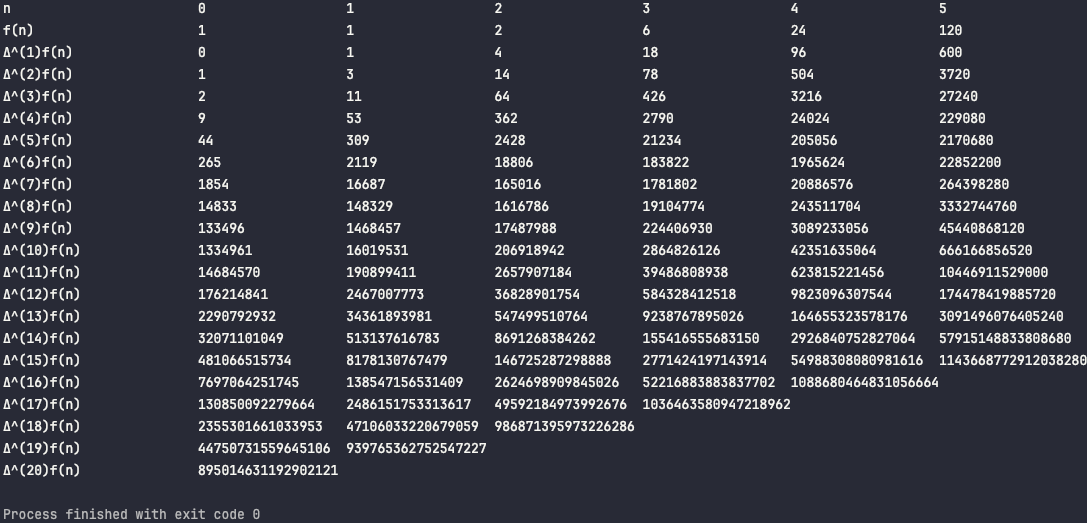
\includegraphics[scale=0.4]{Figures/n_fac_diff.png} \\
        You can clearly see that $D_k$ is the 0th term in all the derivatives. \\
        $$ n! = \sum_{k \geq 0} D_k \binom{n}{k} = \sum_{k \geq 0} \Delta^{(k)} (0)! \binom{n}{k} $$

        Because of linearity we can focus on these two
        $$ D_k = \Delta^{(k)} (0)! $$
        $$ k! \sum_{i = 0}^k \frac{1}{i!} (-1)^i = \Delta^{(k)} (0)! $$
        $$ \sum_{i = 0}^k \frac{1}{i!} (-1)^i = \frac{\Delta^{(k)} (0)!}{k!} $$
        They both converge to $\frac{1}{e}$ therefor they are the same.
        $$ \frac{1}{e} = \frac{1}{e} $$

  
		\item  Examine the difference table for $n!$, and create its discrete Taylor series.

        Look at the difference table in 14 part 1. 

        $$ n! = \sum_{k \geq 0} D_k \binom{n}{k} $$


  
		\item Examine the difference table for $d_n = (-1)^n D_n$, and derive a closed formula for $D_n$ (which you already know from Problem 13). 

        The difference table for $d_n = (-1)^n D_n$ \\
        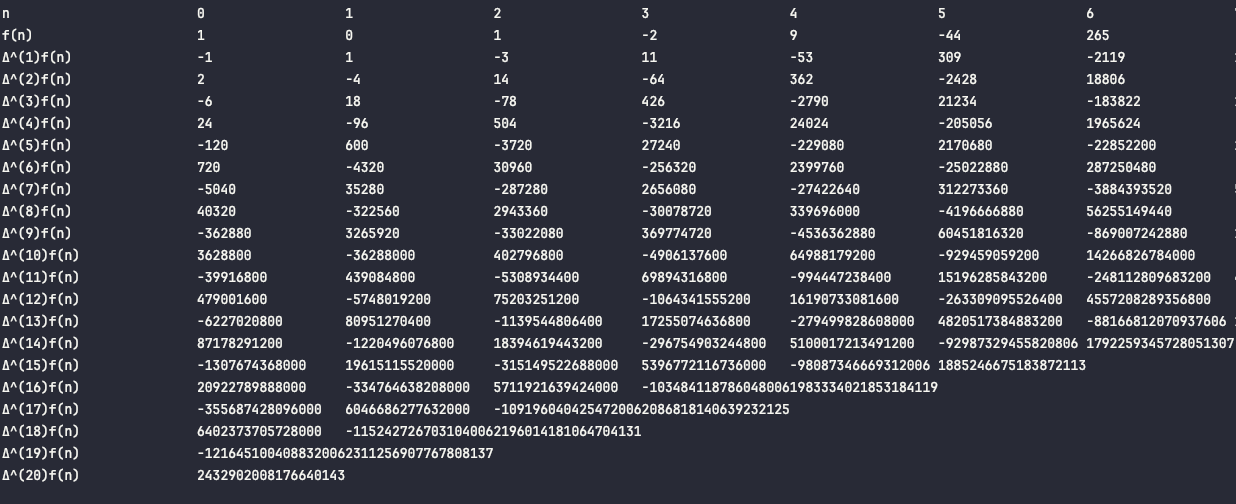
\includegraphics[scale=0.4]{Figures/dn_diff_table.png} \\
        Well if you take the all the derivatives evaluated at 0 and raise them to the $-1$ and sum them all up they will clearly converge to $\frac{1}{e}$. 
        
        $$ n! = (-1)^n \Delta^{(n)} d_0 $$
        $$ \frac{1}{e} = \sum_{n \geq 0} (\Delta^{(n)}d_0)^{-1} $$

        $$ (-1)^n n! = \Delta^{(n)} d_0 $$
        $$ \frac{1}{e} = \sum_{n \geq 0} ((-1)^n n!)^{-1} $$

        $$ \frac{n!}{e} = n! \sum_{n \geq 0} ((-1)^n n!)^{-1} $$
        $$ \lfloor \frac{n!}{e} + \frac{1}{2} \rfloor = \lfloor \frac{1}{2}  + n! \sum_{n \geq 0} ((-1)^n n!)^{-1} \rfloor $$
        Well hey that is $D_n$ \\
        $$ D_n = \lfloor \frac{n!}{e} + \frac{1}{2} \rfloor = \lfloor \frac{1}{2}  + n! \sum_{n \geq 0} ((-1)^n n!)^{-1} \rfloor $$
        




  
	\end{enumerate}
\end{document}